\documentclass[../../spr.tex]{subfiles}

\begin{document}


\section{Implementacja}

\subsection{Opis głównych funkcjonalności aplikacji}

\begin{itemize}
  \item autoryzacja z wykorzystaniem OIDC.
  \item Płatności.
  \item zarządzanie siłownnią
\end{itemize}

\subsection{Prezentacja zrzutów ekranu (screeny) prezentujących działanie aplikacji}
\begin{figure}[H]
  \centering
  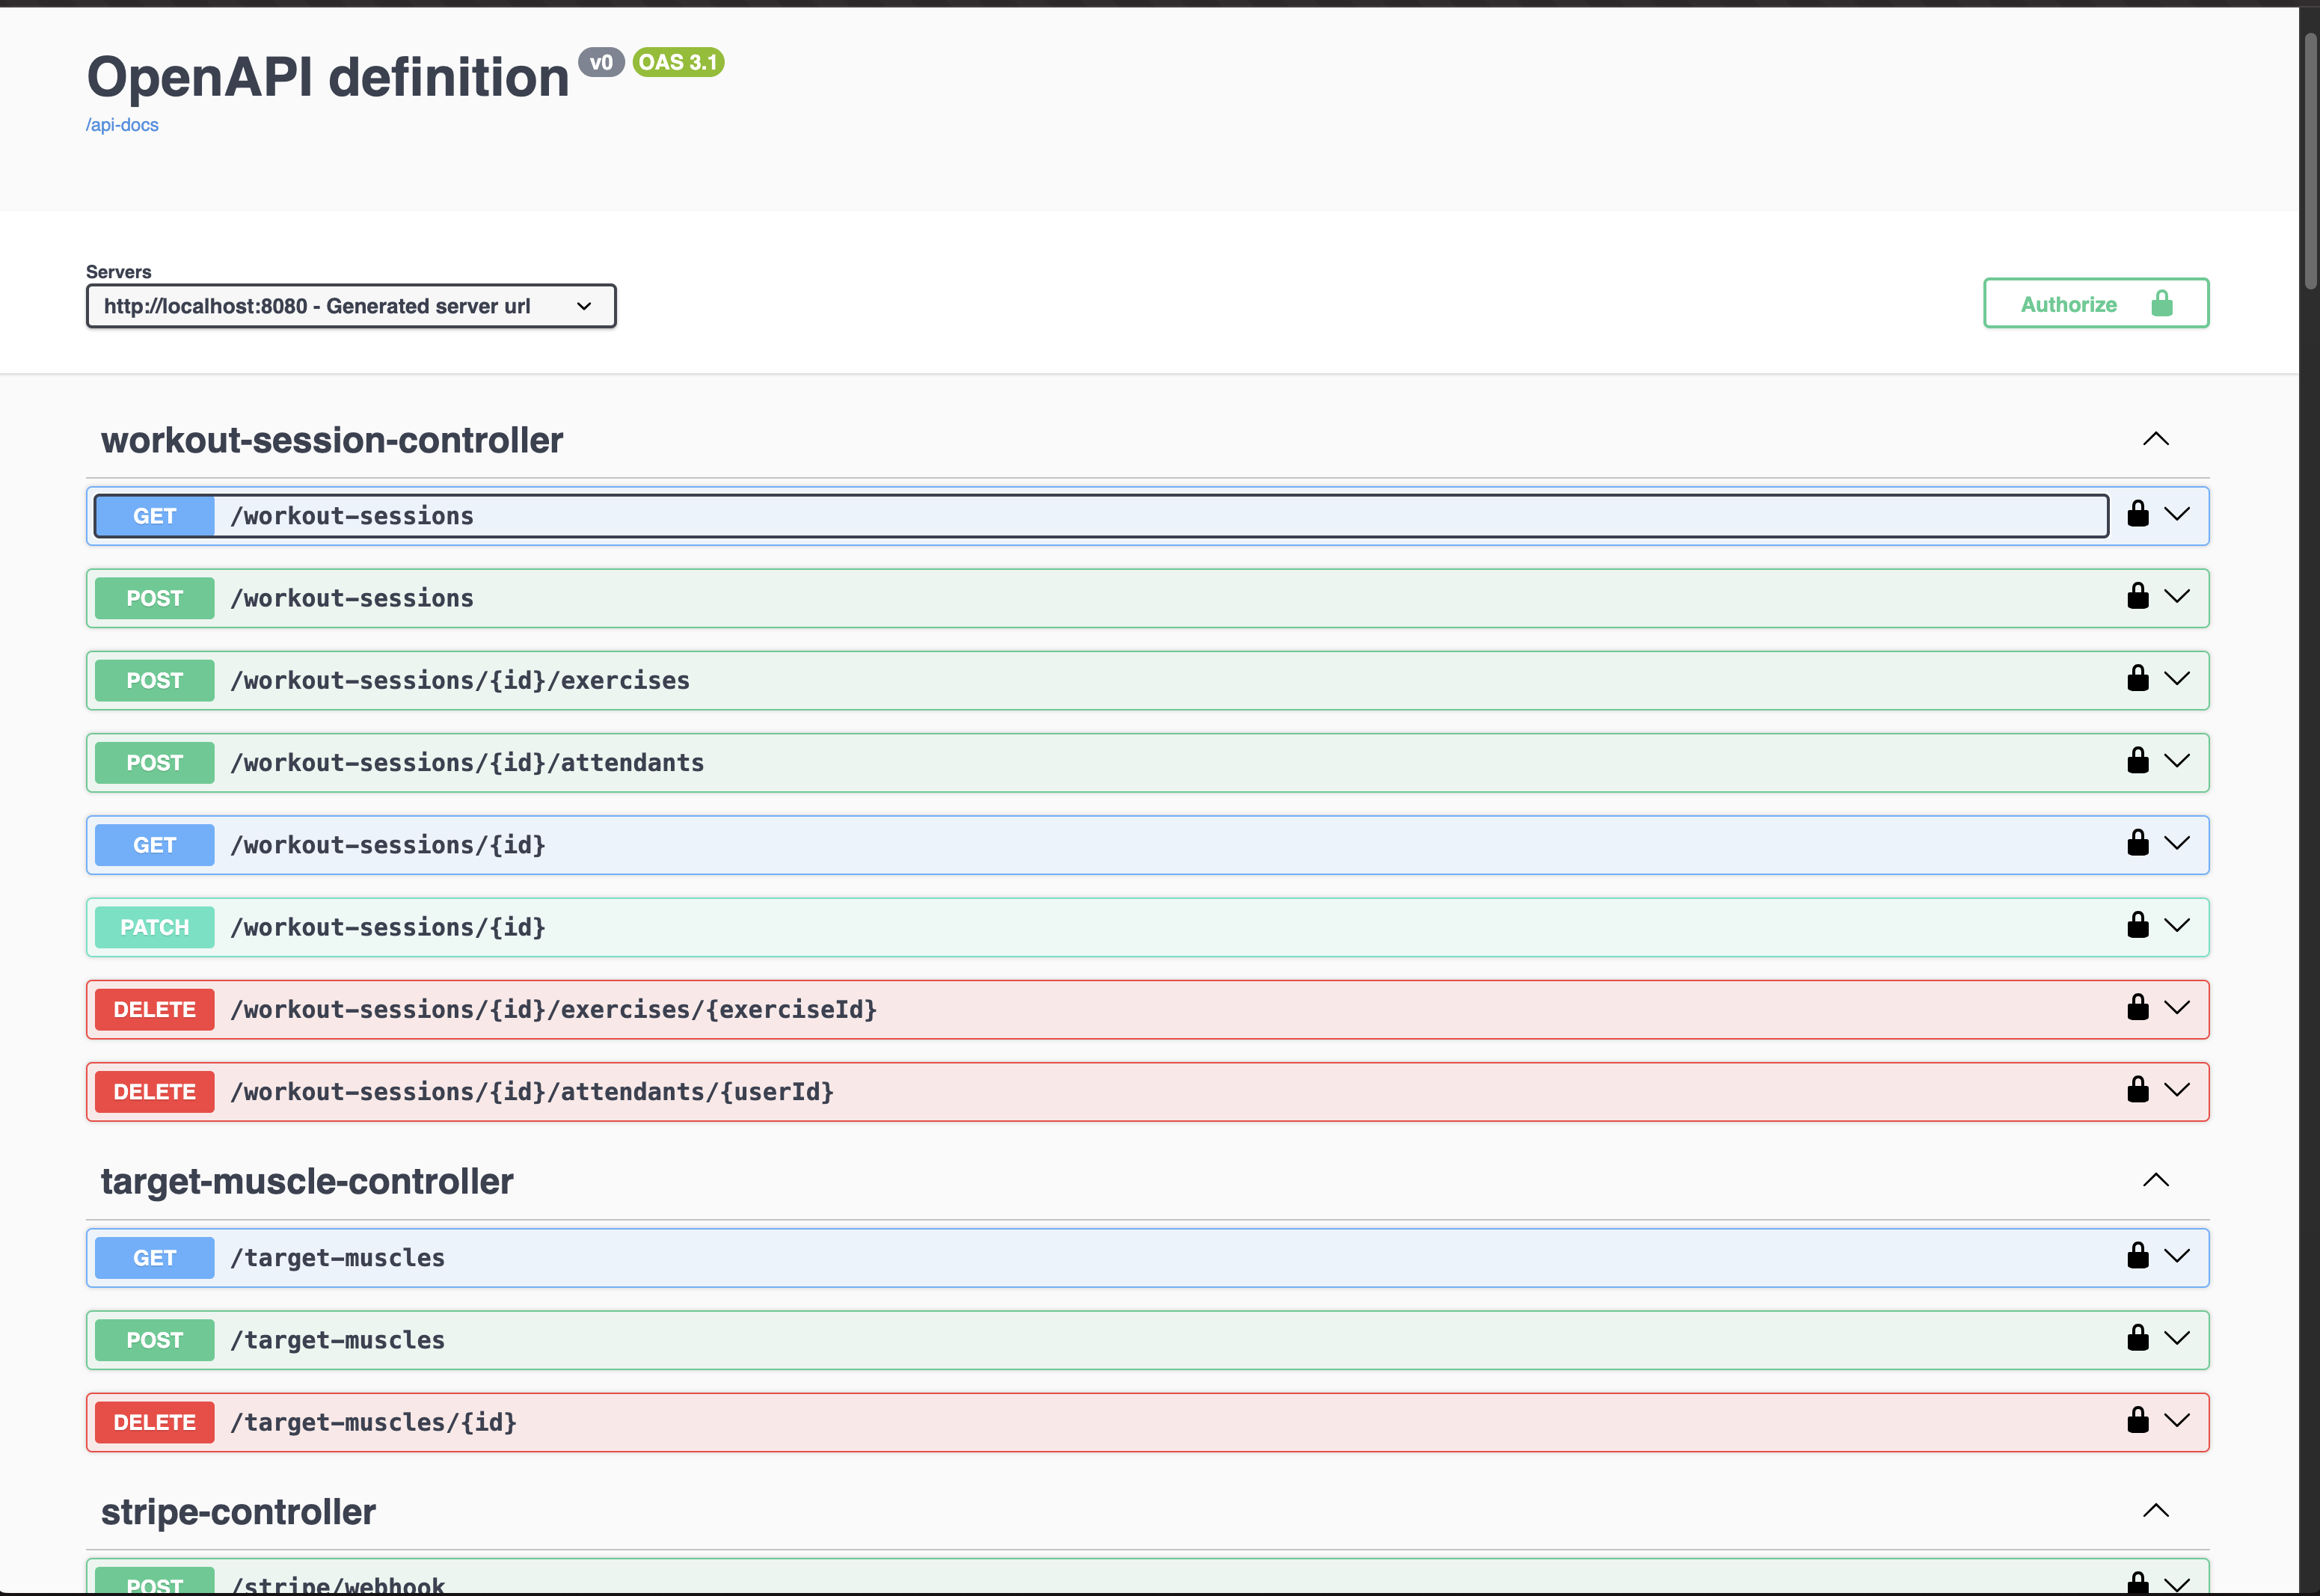
\includegraphics[width=\textwidth]{swagger.png}
  \caption{Swagger UI z dokumentacją API}
\end{figure}

\subsection{Wybrane fragmenty kodu z kluczowymi funkcjonalnościami}


\subsubsection{Autoryzacja z tokena JWT}

Obsługę autoryzacji z tokena JWT przedstawia \cref{auth_jwt}

\begin{listing}
  \inputminted[breaklines, fontsize=\footnotesize, breakanywhere, firstline=18, numbers=left]
  {java}{./sections/implementacja/GymJwtAuthenticationConverter.java}
  \caption{Autoryzacja z tokena JWT OIDC}
  \label{auth_jwt}
\end{listing}

\subsubsection{}

\end{document}